\section{Описание микросхем}

Приведем перечень некоторых электрических параметров интегральных микросхем, их буквенные обозначения и определения, установленные ГОСТ 19480-74 “Микросхемы интегральные. Электрические параметры. Термины, определения и буквенные обозначения”, ГОСТ 18683-73 “Микросхемы интегральные логические. Методы измерения электрических параметров”, ГОСТ 19799-74 “Микросхемы интегральные аналоговые. Методы измерения электрических параметров и определения характеристик”. Затем по этим параметрам дадим характеристику микросхемам, используемым в схеме устройства, а именно микросхемам:

\begin{itemize}
	\item К1114ЕУ4
	\item К176ИЕ12
	\item К561ТМ2
	\item К176ИЕ5
	\item К561ЛЕ10
	\item К561ЛА7
\end{itemize}

\subsection*{Электрические параметры микросхем}

\textbf{Ток потребления I\SB{пот}} \longndash значение тока, потребляемого микросхемой от источников питания в заданном режиме. 

\textbf{Ток потребления в состоянии логического нуля I\SPSB{0}{пот}.} 

\textbf{Ток потребления в состоянии логической единицы I\SPSB{1}{пот}.} 

\textbf{Напряжение логического нуля U\SB{0}} \longndash значение низкого уровня напряжения для “положительной” логики и значение высокого уровня напряжения для “отрицательной” логики. 

\textbf{Напряжение логической единицы U\SB{1}} – значение высокого уровня напряжения для “положительной” логики и значение низкого уровня напряжения для “отрицательной” логики. 

\textbf{Входной ток логического нуля I\SPSB{0}{вх}.}

\textbf{Входной ток логической единицы I\SPSB{0}{вх}.}

\textbf{Ток утечки на входе I\SB{ут, вх}} \longndash значение тока во входной цепи микросхемы при закрытом состоянии входа и заданных режимах на остальных выводах.
 
\textbf{Время задержки распространения сигнала при включении t\SPSB{1,0}{зд, p}} \longndash интервал времени между входным и выходным импульсами при переходе напряжения на выходе микросхемы от напряжения логической единицы к напряжению логического нуля, измеренный на уровне 0,5 или на заданных значениях напряжения.

\textbf{Время задержки распространения сигнала при выключении  t\SPSB{0,1}{зд, p}} \longndash интервал времени между входным и выходным импульсами при переходе напряжения на выходе микросхемы от напряжения логического нуля к напряжению логической единицы, измеренный на уровне 0,5 или на заданных значениях напряжения. 

\textbf{Помехоустойчивость статическая U\SB{п, ст}} \longndash наибольшее значение допустимого напряжения статической помехи по высокому и низкому уровням входного напряжения, при котором еще не происходит изменение уровней выходного напряжения цифровой интегральной микросхемы. 

\textbf{Коэффициент разветвления по выходу K\SB{раз}} \longndash число единичных нагрузок, которое можно одновременно подключить к выходу микросхемы (единичной нагрузкой является один вход основного логического элемента данной серии интегральных микросхем).

\subsection*{К1114ЕУ4}

Микросхема представляет собой многофункциональную схему управления источником вторичного электропитания (двухтактный ШИМ-контроллер). ИС осуществляет формирование опорного напряжения, усиление сигнала ошибки, формирование пилообразного напряжения, ШИМ-модуляцию, формирование 2-тактного выхода, защиту сквозных токов, защиту от перегрузок, включение и выключение, внешнюю синхронизацию, формирование частотной характеристики и обеспечение мягкого запуска. Корпус типа 238.16-2, масса не более 1,5 г.

\begin{figure}[ht]
  \center{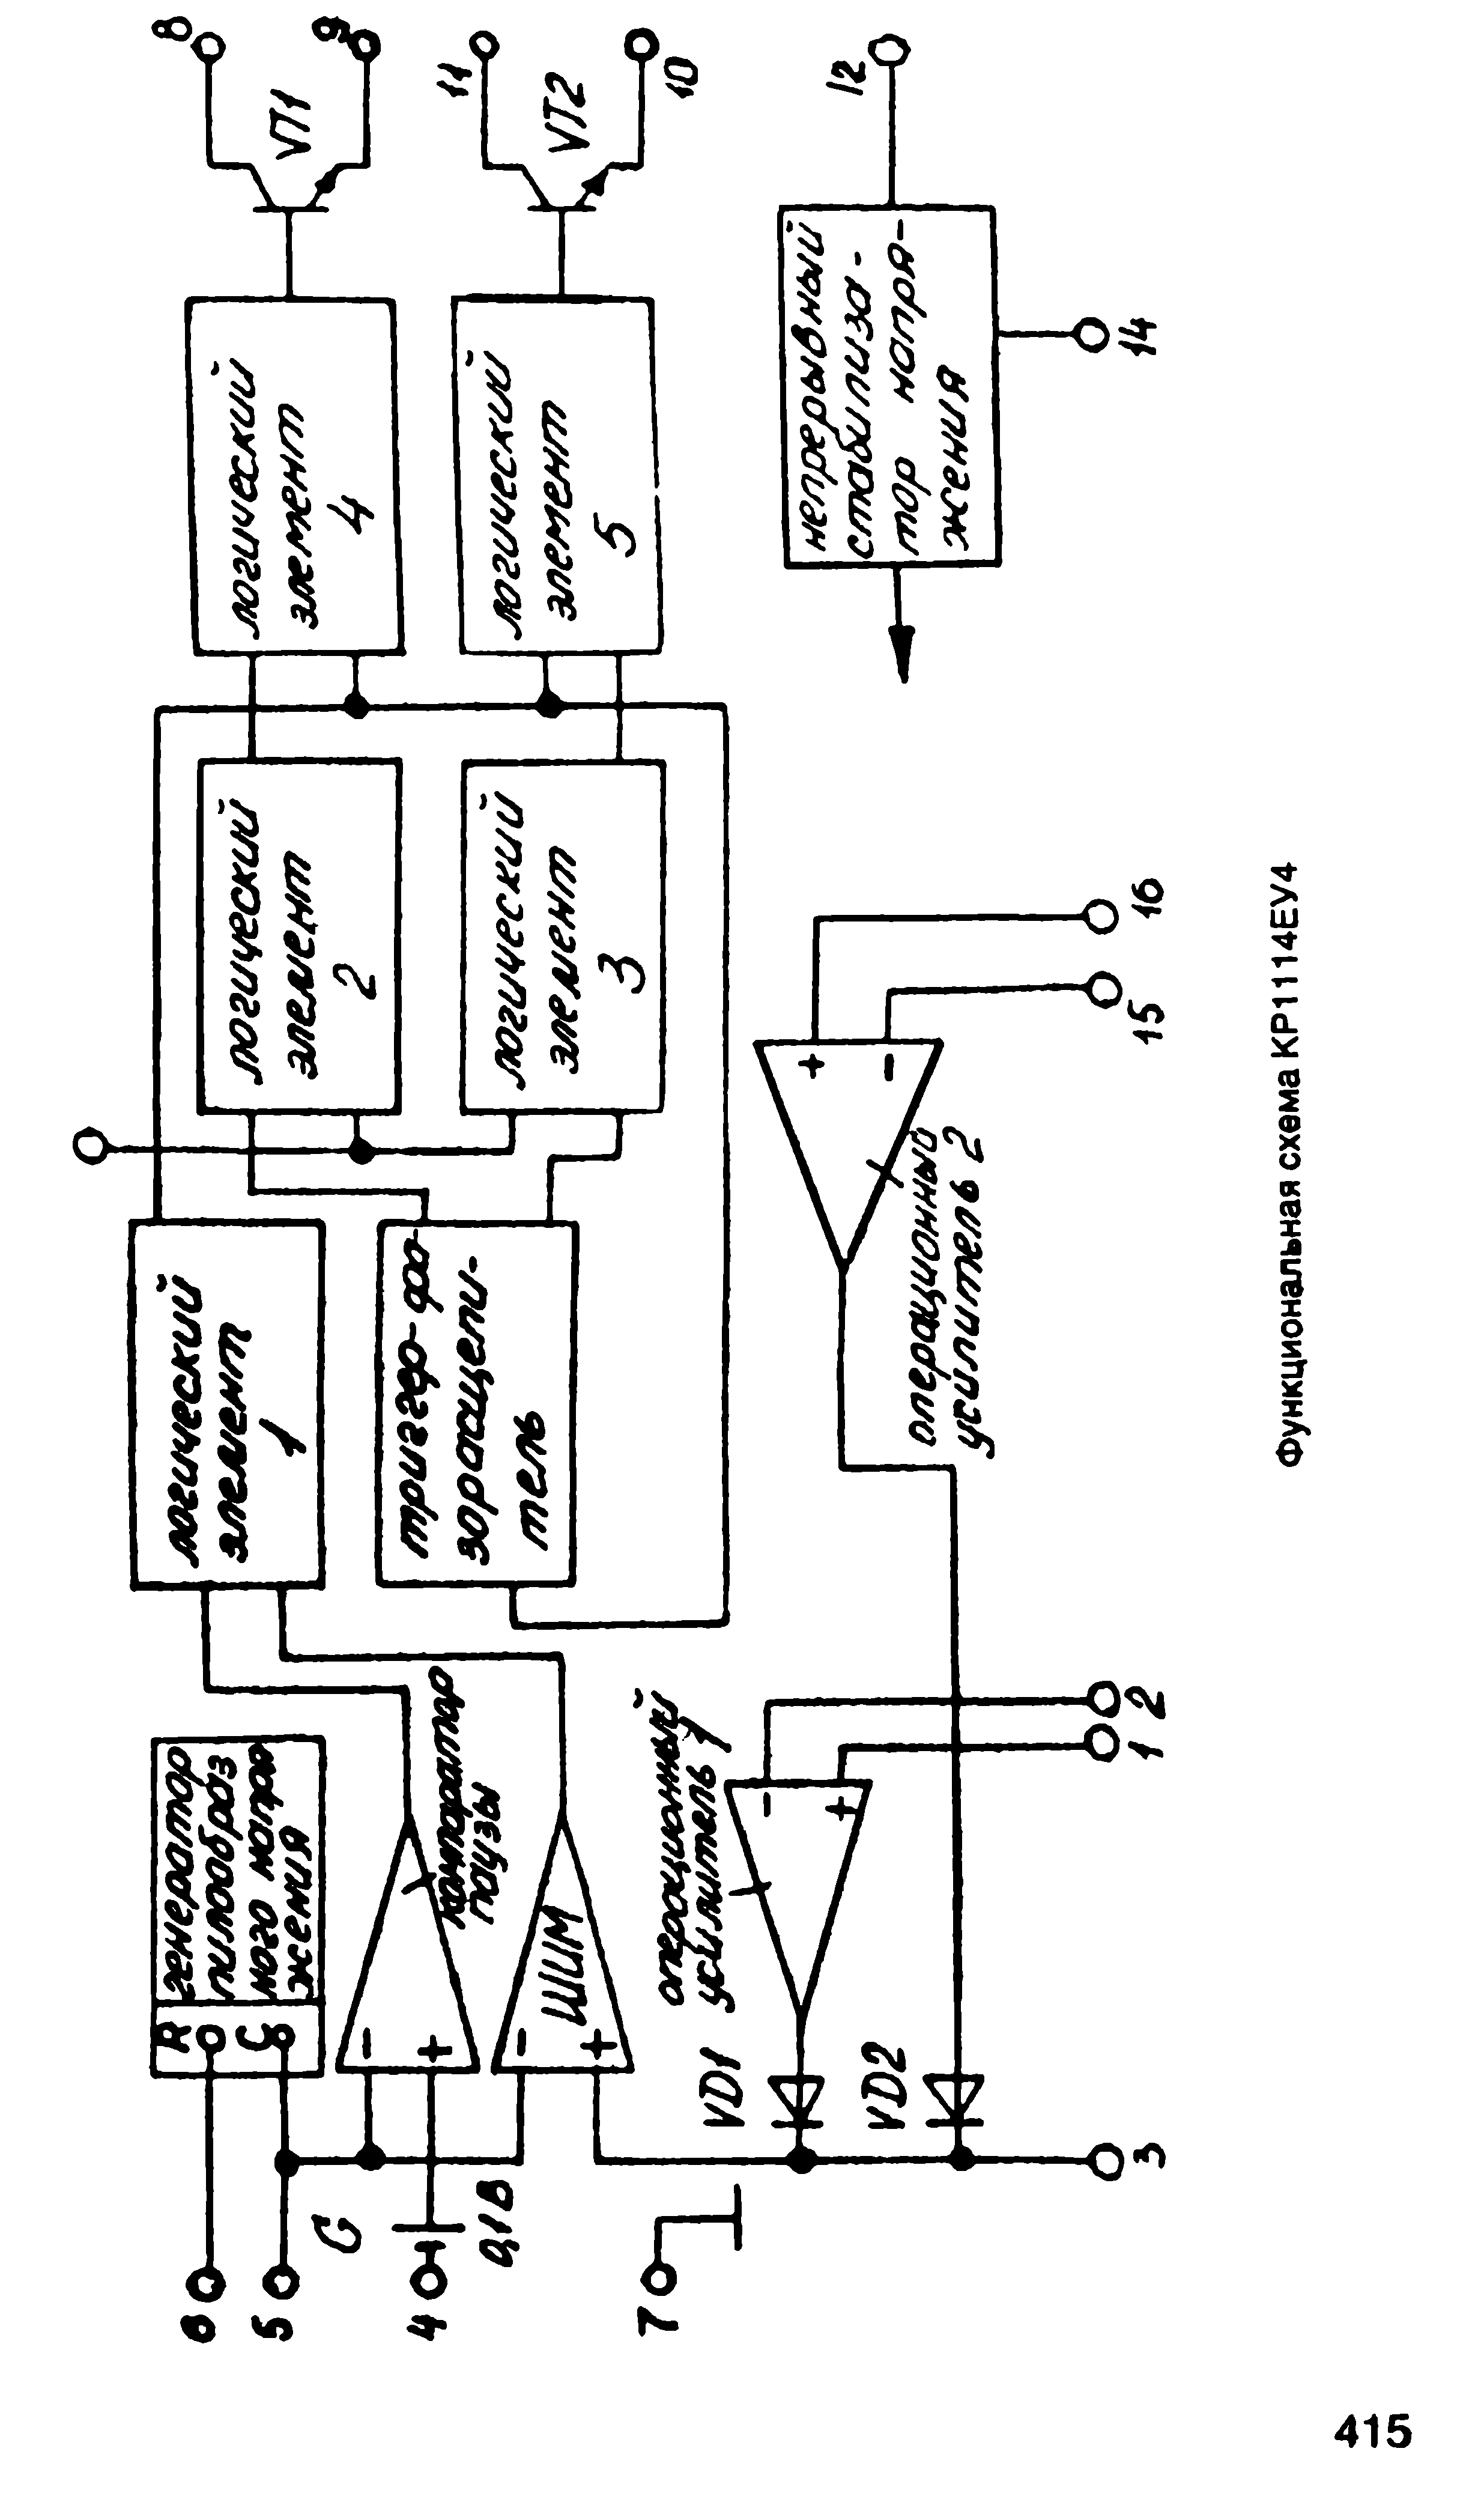
\includegraphics[width=0.5\textwidth]{Images/К1114ЕУ4.png}}
  
  \caption{Условно-графическое обозначение К1114ЕУ4}
  \label{img:k1114eu4}
\end{figure}

Назначение выводов:
1 \longndash неинвертирующий вход ОУ 1;
2 \longndash интвертирующий вход ОУ 1;
3 \longndash выход усилителей;
4 \longndash установка паузы;
5 \longndash вход для подключения конденсатора задания частоты;
6 \longndash вход для подключения резистора задания частоты;
7 \longndash общий;
8 \longndash коллектор VT1;
9 \longndash эмиттер VT1;
10 \longndash эмиттер VT2;
11 \longndash коллектор VT2;
12 \longndash напряжение питания;
13 \longndash блокировка двухтактного выхода;
14 \longndash выход источника опорного напряжения;
15 \longndash инвертирующий вход ОУ 2;
16 \longndash неинвертирующий вход ОУ 2; 

\subsubsection*{Электрические параметры}
\begin{itemize}
	\item[] Номинальное напряжение питания \dotfill $12~\text{В} \pm 5\%$
	\item[] Остаточное напряжение \dotfill $\leq 1,3~\text{В}$
	\item[] Опорное напряжение \dotfill $4,5..5,5~\text{В}$
	\item[] Ток потребления \dotfill $\leq 20~\text{мА}$
	\item[] Ток закрытой микросхемы \dotfill $\leq 100~\text{мкА}$
	\item[] Длительность фронта импульса выходного тока \dotfill $\leq 100~\text{нс}$
	\item[] Длительность среза импульса выходного тока \dotfill $\leq 200~\text{нс}$
	\item[] Температурный коэффицинт опорного напряжения \dotfill $\leq 0,03 \%/\degree C$
	\item[] Нестабильность по напряжению источника опорного напряжения \dotfill $\leq 0,05\%$
	\item[] Нестабильность по току источника опорного напряжения \dotfill $\leq 1\%$
\end{itemize}

\subsection*{К176ИЕ12}

Микросхема представляет собой двоичный счётчик на 60 и 15-разрядный делитель частоты. Содержит 696 интегральных элементов. Корпус типа 238.16-1 и типа 2103.16-11, масса не более 1,5 г. \\

\begin{figure}[ht]
  \center{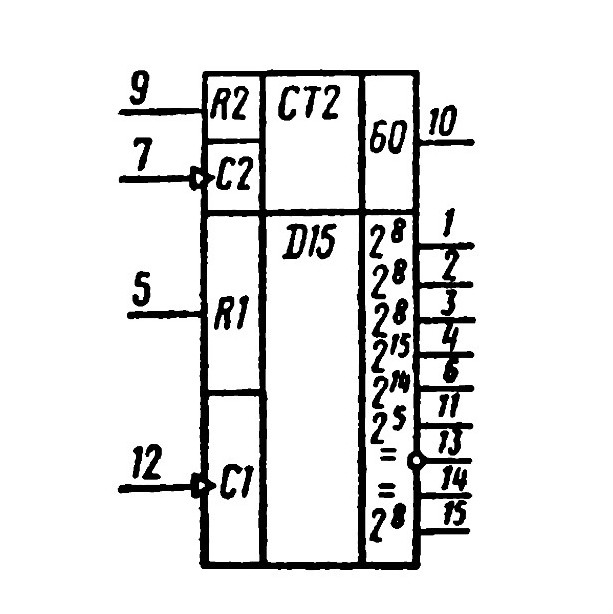
\includegraphics[width=0.3\textwidth]{Images/К176ИЕ12.png}}
  
  \caption{Условно-графическое обозначение К176ИЕ12}
  \label{img:k176ie12}
\end{figure}

Назначение выводов: 1 \longndash выход мультиплексора (2\SP{6}), T2; 2 \longndash выход мультиплексора 2\SP{3}, T4; 3 \longndash выход мультиплексора 2\SP{6}, T1; 4 \longndash выход делителя 2\SP{15}; 5 \longndash вход установка "0" делителя R1; 6 \longndash выход делителя 2\SP{14}; 7 \longndash вход счётчика C2; 8 \longndash общий; 9 \longndash вход установка "0" счётчика, R2; 10 \longndash выход счётчика; 11 \longndash выход делителя 2\SP{5}; 12 \longndash вход делителя C1; 13 \longndash выход делителя (=) инверсный; 14, 15 \longndash выходы делителя; 16 \longndash напряжение питания.

\subsubsection*{Электрические параметры}
\begin{itemize}
	\item[] Номинальное напряжение питания \dotfill $9~\text{В} \pm 5\%$
	\item[] Выходное напряжение низкого уровня \dotfill $\leq 0,3~\text{В}$
	\item[] Выходное напряжения высокого уровня \dotfill $\geq 8,2~\text{В}$
	\item[] Входной ток низкого уровня \dotfill $\geq -0,3~\text{мкА}$
	\item[] Входной ток высокого уровня \dotfill $\leq 0,3~\text{мкА}$
	\item[] Ток потребления \dotfill $\leq 25~\text{мкА}$
	\item[] Ток потребления в динамическом режиме \dotfill $\leq 0,3~\text{мА}$
	\item[] Мощность потребления \dotfill $\leq 50~\text{мВт}$
	\item[] Частота тактовых сигналов \dotfill $\geq 1,2~\text{МГц}$
	\item[] Входная емкость \dotfill $\leq 10~\text{пФ}$
	\item[] Коэффициент разветвления по выходу \dotfill $\leq 50$
\end{itemize}

\subsection*{К561ТМ2}

Микросхема представляет собой два D-триггера с динамическим управлением. Установка триггера по входам R и S принудительная, поэтому сигналы синхронизации C и информационного входа D не изменяют состояния триггера на выходе во время действия сигналов R и S. Содержит 128 интегральных элементов. Корпус типа 201.14-1, масса не более 1 г и 4306.14-А.

\begin{figure}[ht]
  \center{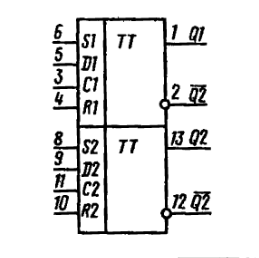
\includegraphics[width=0.25\textwidth]{Images/К561ТМ2.png}}
  
  \caption{Условно-графическое обозначение К561ТМ2}
  \label{img:k561tm2}
\end{figure}

Назначение выводов: 1 \longndash выход $Q1$; 2 \longndash выход $\bar{Q1}$; 3 \longndash вход $C1$; 4 \longndash вход $R1$; 5 \longndash вход $D1$; 6 \longndash вход $S1$; 7 \longndash общий; 8 \longndash вход $S2$; 9 \longndash вход $D2$; 10 \longndash вход $R2$; 11 \longndash вход $C2$; 12 \longndash выход $\bar{Q2}$; 13 \longndash выход $Q2$; 14 \longndash напряжение питания.

\begin{figure}[ht]
  \center{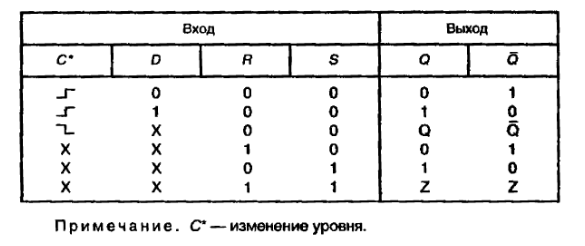
\includegraphics[width=0.8\textwidth]{Images/truthtable.png}}
  
  \caption{Таблица истинности К561ТМ2}
  \label{img:truthtable}
\end{figure}

\subsubsection*{Электрические параметры}
\begin{itemize}
    \item[] Напряжение питания \dotfill $3...15~\text{В}$
    \item[] Выходное напряжение низкого уровня при воздействии помехи:
    \begin{itemize}
	    \item[] при $U_{\text{п}}=5~\text{В}$ \dotfill $\leq 0,8~\text{В}$
	    \item[] при $U_{\text{п}}=10~\text{В}$ \dotfill $\leq 1~\text{В}$
    \end{itemize}
    \item[] Выходное напряжения высокого уровня при воздействии помехи: 
    \begin{itemize}
	    \item[] при $U_{\text{п}}=5~\text{В}$ \dotfill $\geq 4,2~\text{В}$ 
	    \item[] при $U_{\text{п}}=10~\text{В}$ \dotfill $\geq 9~\text{В}$
    \end{itemize}
    \item[] Ток потребления при $U_{\text{п}}=15~\text{В}$ \dotfill $\leq 25~\text{мкА}$
    \item[] Входной ток низкого (высокого) уровня при $U_{\text{п}}=15~\text{В}$  \dotfill $\leq -0,3~\text{мкА}$
    \item[] Выходной ток низкого уровня: 
    \begin{itemize}
	    \item[] при $U_{\text{п}}=5~\text{В}$ \dotfill $\geq 0,5~\text{мА}$ 
	    \item[] при $U_{\text{п}}=10~\text{В}$ \dotfill $\geq 0,9~\text{мА}$
    \end{itemize}
    \item[] Выходной ток высокого уровня: 
    \begin{itemize}
	    \item[] при $U_{\text{п}}=5~\text{В}$ \dotfill $\geq 0,25~\text{мА}$ 
	    \item[] при $U_{\text{п}}=10~\text{В}$ \dotfill $\geq 0,6~\text{мА}$
    \end{itemize}
    \item[] Время задержки распространения при включении (выключении): 
    \begin{itemize}
	    \item[] при $U_{\text{п}}=5~\text{В}$ \dotfill $\leq 420~\text{нс}$ 
	    \item[] при $U_{\text{п}}=10~\text{В}$ \dotfill $\leq 150~\text{нс}$
    \end{itemize}
    \item[] Входная емкость при $U_{\text{п}}=10~\text{В}$ \dotfill $\leq 10~\text{пФ}$
\end{itemize}


\subsection*{К176ИЕ5}

Микросхема представляет собой 15-разрядный двоичный делитель частоты. Содержит 307 интегральных элементов. Корпус типа 2102.14-4 и типа 201.14-1, масса не более 1 г.

\begin{figure}[ht]
  \center{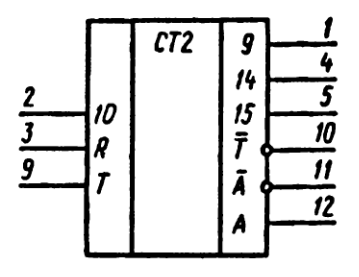
\includegraphics[width=0.3\textwidth]{Images/К176ИЕ5.png}}
  
  \caption{Условно-графическое обозначение К176ИЕ5}
  \label{img:k176ie5}
\end{figure}

Назначение выводов: 1 \longndash выход 9 разряда; 2 \longndash выход 10 разряда; 3 \longndash вход установки "0" R; 4 \longndash выход 14 разряда; 5 \longndash выход 15 разряда; 6,7 \longndash общие; 8, 13 \longndash свободные; 9 \longndash вход $T$; 10 \longndash выход $\bar{T}$; 11 \longndash выход $\bar{A}$; 12 \longndash выход $A$; 14 \longndash напряжение питания.

\subsubsection*{Электрические параметры}
\begin{itemize}
	\item[] Номинальное напряжение питания \dotfill $9~\text{В} \pm 5\%$
	\item[] Выходное напряжение низкого уровня \dotfill $\leq 0,3~\text{В}$
	\item[] Выходное напряжения высокого уровня \dotfill $\geq 8,2~\text{В}$
	\item[] Входной ток низкого уровня \dotfill $\geq -0,5~\text{мкА}$
	\item[] Входной ток высокого уровня \dotfill $\leq 0,5~\text{мкА}$
	\item[] Ток потребления \dotfill $\leq 0,25~\text{мкА}$
	\item[] Ток потребления в динамическом режиме \dotfill $\leq 0,3~\text{мА}$
	\item[] Максимальная мощность \dotfill $\leq 21~\text{мВт}$
	\item[] Тактовая частота деления \dotfill $\geq 1~\text{МГц}$
	\item[] Нагрузочная способность в статическом режиме \dotfill $\leq 15$
\end{itemize}

\subsection*{К561ЛЕ10}

Микросхема представляет собой три трехвходовых элемента ИЛИ-НЕ. Содержат 54 интегральных элемента. Корпус типа 201.14-1, масса не более 1 г, и 4306.14-А.

\begin{figure}[ht]
  \center{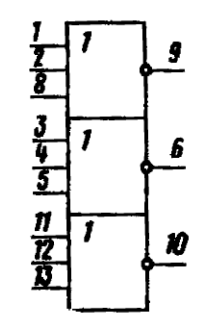
\includegraphics[width=0.2\textwidth]{Images/К561ЛЕ10.png}}
  
  \caption{Условно-графическое обозначение К561ЛЕ10}
  \label{img:k561le10}
\end{figure}

Назначение выводов: 1,2,3,4,5,7,11,12,13 \longndash входы; 6,9,10 \longndash выходы; 7 \longndash общий; 14 \longndash напряжение питания.

\subsubsection*{Электрические параметры}
\begin{itemize}
	\item[] Напряжение питания \dotfill $3...15~\text{В}$
	\item[] Выходное напряжение низкого уровня \dotfill $\leq 0,01~\text{В}$
	\item[] Максимальное выходное напряжения низкого уровня \dotfill $\leq 2,9~\text{В}$
	\item[] Минимальное выходное напряжения высокого уровня \dotfill $\geq 7,2~\text{В}$
	\item[] Ток потребления \dotfill $\leq 5~\text{мкА}$
	\item[] Входной ток низкого уровня \dotfill $\leq|-0,05|~\text{мкА}$
	\item[] Входной ток высокого уровня \dotfill $\leq 0,05~\text{мкА}$
	\item[] Выходной ток низкого уровня \dotfill $\geq 0,6~\text{мА}$
	\item[] Выходной ток высокого уровня \dotfill $\geq|-0,25|~\text{мА}$
	\item[] Ток потребления в динамическом режиме \dotfill $\leq 0,3~\text{мА}$
	\item[] Время задержки распр. входного сигнала при включении \dotfill $\leq 125~\text{нс}$
	\item[] Время задержки распр. входного сигнала при выключении \dotfill $\leq 145~\text{нс}$
\end{itemize}

\subsection*{К561ЛА7}

Микросхема представляет собой четыре логических элемента 2И-НЕ. Содержат 64 интегральных элемента. Корпус типа 201.14-1, масса не более 1 г и 4306.14-А.

\begin{figure}[ht]
  \center{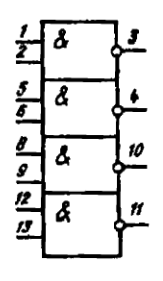
\includegraphics[width=0.2\textwidth]{Images/К561ЛА7.png}}
  
  \caption{Условно-графическое обозначение К561ЛА7}
  \label{img:k561la7}
\end{figure}

Назначение выводов: 1 \longndash вход $X2$; 2 \longndash вход $X1$; 3 \longndash выход $Y1$; 4 \longndash выход $Y2$; 5 \longndash вход $X3$; 6 \longndash вход $X4$; 7 \longndash общий; \longndash вход $X6$; 9 \longndash вход $X5$; 10 \longndash выход $Y3$; 11 \longndash выход $Y4$; 12 \longndash вход $X7$; 13 \longndash вход $X8$; 14 \longndash напряжение питания.

\subsubsection*{Электрические параметры}
\begin{itemize}
    \item[] Напряжение питания \dotfill $3...15~\text{В}$
    \item[] Выходное напряжение низкого уровня при воздействии помехи:
    \begin{itemize}
	    \item[] при $U_{\text{п}}=10~\text{В}$ \dotfill $\leq 2,9~\text{В}$
	    \item[] при $U_{\text{п}}=5~\text{В}$ \dotfill $\leq 0,95~\text{В}$
    \end{itemize}
    \item[] Выходное напряжения высокого уровня при воздействии помехи при $U_{\text{п}}=10~\text{В}$ \dotfill $\geq 7,2~\text{В}$
    \item[] Ток потребления при $U_{\text{п}}=15~\text{В}$ \dotfill $\leq 5~\text{мкА}$
    \item[] Входной ток низкого (высокого) уровня при $U_{\text{п}}=15~\text{В}$  \dotfill $\leq -0,3~\text{мкА}$
    \item[] Выходной ток низкого уровня: 
    \begin{itemize}
	    \item[] при $U_{\text{п}}=10~\text{В}$ \dotfill $\geq 1,3~\text{мА}$ 
	    \item[] при $U_{\text{п}}=5~\text{В}$ \dotfill $\geq 0,51~\text{мА}$
    \end{itemize}
    \item[] Выходной ток высокого уровня: 
    \begin{itemize}
	    \item[] при $U_{\text{п}}=10~\text{В}$ \dotfill $\geq 1,3~\text{мА}$ 
	    \item[] при $U_{\text{п}}=5~\text{В}; U_{\text{вых}}=4,6~\text{В}$ \dotfill $\geq 0,51~\text{мА}$
	    \item[] при $U_{\text{п}}=5~\text{В}; U_{\text{вых}}=2,5~\text{В}$ \dotfill $\geq 1,6~\text{мА}$
    \end{itemize}
    \item[] Время задержки распространения при включении (выключении): 
    \begin{itemize}
	    \item[] при $U_{\text{п}}=10~\text{В}$ \dotfill $\leq 80~\text{нс}$ 
	    \item[] при $U_{\text{п}}=5~\text{В}$ \dotfill $\leq 160~\text{нс}$
    \end{itemize}
    \item[] Входная емкость \dotfill $\leq 11~\text{пФ}$
\end{itemize}